% Chapter 5
\chapter{Evaluation}\label{ch:eval}
To evaluate the proposed method two classes of experiments are carried out. In a first step an example planner is implemented which mimics the local planning step and provides an easy way to test the trajectory evaluation separated from the rest of a conventional planning system.

With the gained data the algorithms are improved and used to extend existing local planner. A fully simulated environment and robotic model using a sophisticated physic engine together with a complete robot navigation system is used to compare the original implementation of the local planner with the meta-heuristic approach.
 
\section{Experiments with sample planner}
The trajectory sampling and selection of a common DWA approach are implemented in python minimizing a simpler cost function $f_c(v,w)$ (cf. Equation~\ref{eq:simplecost}), where $f_g(v,w)$ is the distance of the center of the robot in the end position to a predefined goal position, and $f_o(v,w)$ is the maximal distance to an obstacle on the trajectory path.

\begin{equation}
   f_c(v,w)=\alpha f_g(v,w) - \beta f_o(v,w)
   \label{eq:simplecost}
\end{equation}

To select a benchmark cost a brute force search is performed on random generated test instances, evaluating a fixed number of trajectories. 
The time the algorithm needs to find this benchmark solution is used to compare their performance.

All algorithm are tested using different minimal, and maximal velocities to account for different acceleration limits. 

The weighting coefficients of the cost function are fixed in our case to $\alpha=0.01$ and $\beta=1$. The local goal is also at a fixed location in the map. 
The step size of the collision test is fixed to 0.015 meter. 
Forward simulation time is fixed to one second. 

The following 60 test instances include different obstacle counts and random placement of quadratic obstacles:
\begin{itemize}
\item 15 instances with 1 obstacle and side length 1 meter.
\item 15 instances with 3 obstacles and side length 1 meter.
\item 15 instances with 5 obstacles and side length 0.5 meter.
\item 15 instances with 25 obstacles and side length 0.1 meter.
\end{itemize}

The instances simulate a snapshot of the local environment of the robot at a given time point, which is used as a local map for input of the local planner.
The resolution of the maps is fixed to 0.05 meter/pixel, resulting in a quadratic map of size 7.5 meter. Figure~\ref{fig:fig_instances} illustrates random instances with differ in size and number of obstacles. 
%\begin{figure}[thpb]
\begin{figure}[thpb]
     \footnotesize
      \centering
      \myfloatalign
      \setlength\fboxsep{0pt}
      \setlength\fboxrule{0.5pt}
       \subfloat[]
       {  
           \fbox{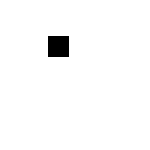
\includegraphics[width=0.3\textwidth]{figures/01_1_b_nocost.png}}
       } 
       \subfloat[]
       {  
           \fbox{
\includegraphics[width=0.3\textwidth]{figures/02_01_1_b_nocost.png}}
       } 
       \subfloat[]
       {  
           \fbox{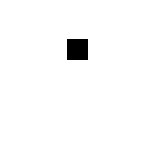
\includegraphics[width=0.3\textwidth]{figures/03_01_1_b_nocost.png}}
       }\\ 
       \subfloat[]
       {  
           \fbox{
\includegraphics[width=0.3\textwidth]{figures/01_02_3_b_nocost.png}}
       } 
       \subfloat[]
       {  
           \fbox{
\includegraphics[width=0.3\textwidth]{figures/02_02_3_b_nocost.png}}
       } 
       \subfloat[]
       {  
           \fbox{
\includegraphics[width=0.3\textwidth]{figures/03_02_3_b_nocost.png}}
       }\\ 
       \subfloat[]
       {  
           \fbox{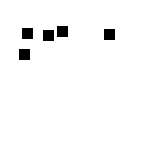
\includegraphics[width=0.3\textwidth]{figures/03_5_m_nocost.png}}
       } 
       \subfloat[]
       {  
           \fbox{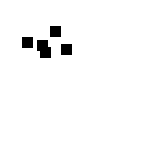
\includegraphics[width=0.3\textwidth]{figures/02_03_5_m_nocost.png}}
       } 
       \subfloat[]
       {  
           \fbox{
\includegraphics[width=0.3\textwidth]{figures/03_03_5_m_nocost.png}}
       }\\
       \subfloat[]
       {  
           \fbox{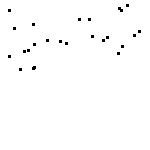
\includegraphics[width=0.3\textwidth]{figures/04_25_s_nocost.png}}
       }      
       \subfloat[]
       {  
           \fbox{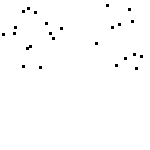
\includegraphics[width=0.3\textwidth]{figures/02_04_25_s_nocost.png}}
       } 
       \subfloat[]
       {  
           \fbox{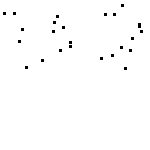
\includegraphics[width=0.3\textwidth]{figures/03_04_25_s_nocost.png}}
       }   
       \caption[Test instances]{Figures (a)-(l) show randomly generated local obstacle maps. The instances differ in number and size of obstacles and are used for local costmap creation. Up to 60 instances are used to evaluate the proposed method.}
      \label{fig:fig_instances}
   \end{figure}

The following list shows the tested algorithm:
\begin{itemize}
\item{\bf{Random Search with Tabu List:}} A repeated random guess of a velocity tuple $(v,w)$ (Random).
\item{\bf{Iterated Local Search:}} Performing Iterated Local Search with 4, 8 ,and 16 neighbors and Tabu List (ILS4, ILS8, ILS16).
\item{\bf{Variable Neighborhood Search:}} Variable Neighborhood search with Best-,and First-Improvement heuristic, and Tabu List (VNSB, VNSF).
\end{itemize}

\section{Experiments extending existing local planner}
To extend an existing local planner the navigation system implemented in the ROS framework is used, which provides a variety of different planning methods. 
The planning system chosen for testing comes ready to use in the implementation of the navigation stack of the ROS framework, which was introduced and implemented by Marder-Eppstein (see \cite{DBLP:conf/icra/Marder-EppsteinBFGK10}).
The local planning system consists of two planners based on \emph{DWA} implementation and \emph{Trajectory Roll-out} (see Section~\ref{sec:dwa}).

To simulate the environment and the robot the simulation framework Gazebo is used, which provides a robust physical engine and is one of the most popular simulation engines in the field of mobile robotics. 

In Figure~\ref{fig:gazebo_v4r} the 3D-model, which is a simple artificial building with four corridors, used for the simulation together with a snapshot of the planning information is depicted.

\begin{figure}[thpb]
     \footnotesize
      \centering
      \myfloatalign
      \setlength\fboxsep{0pt}
      \setlength\fboxrule{0.5pt}
       \subfloat[]
       {  
           \fbox{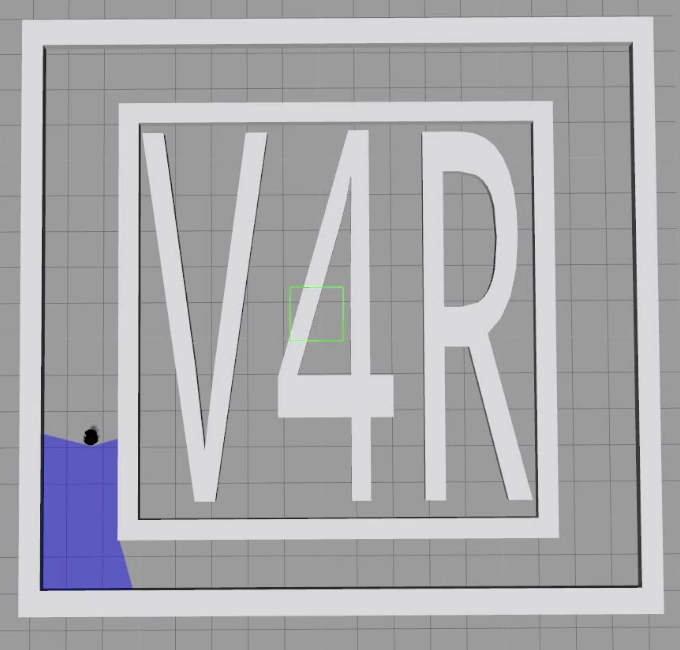
\includegraphics[width=0.85\textwidth]{figures/fig_gazebo_v4r.png}}
       }\\
       \subfloat[]
       {  
           \fbox{
\includegraphics[width=0.85\textwidth]{figures/fig_rviz_v4r.png}}
       }        
       \caption[Simulation: artificial environment]{Figure (a) shows the 3D model of an artificial building used for the experiments with the simulation software Gazebo. Figure (b) depicts planning information used during the experiments.}
      \label{fig:gazebo_v4r}
   \end{figure}

In Figure~\ref{fig:gazebo_gh25} the second 3D-model used for testing is shown. Based on a real map this office environment includes more difficult planning situations, like small doorways and corridors.

\begin{figure}[thpb]
     \footnotesize
      \centering
      \myfloatalign
      \setlength\fboxsep{0pt}
      \setlength\fboxrule{0.5pt}
       \subfloat[]
       {  
           \fbox{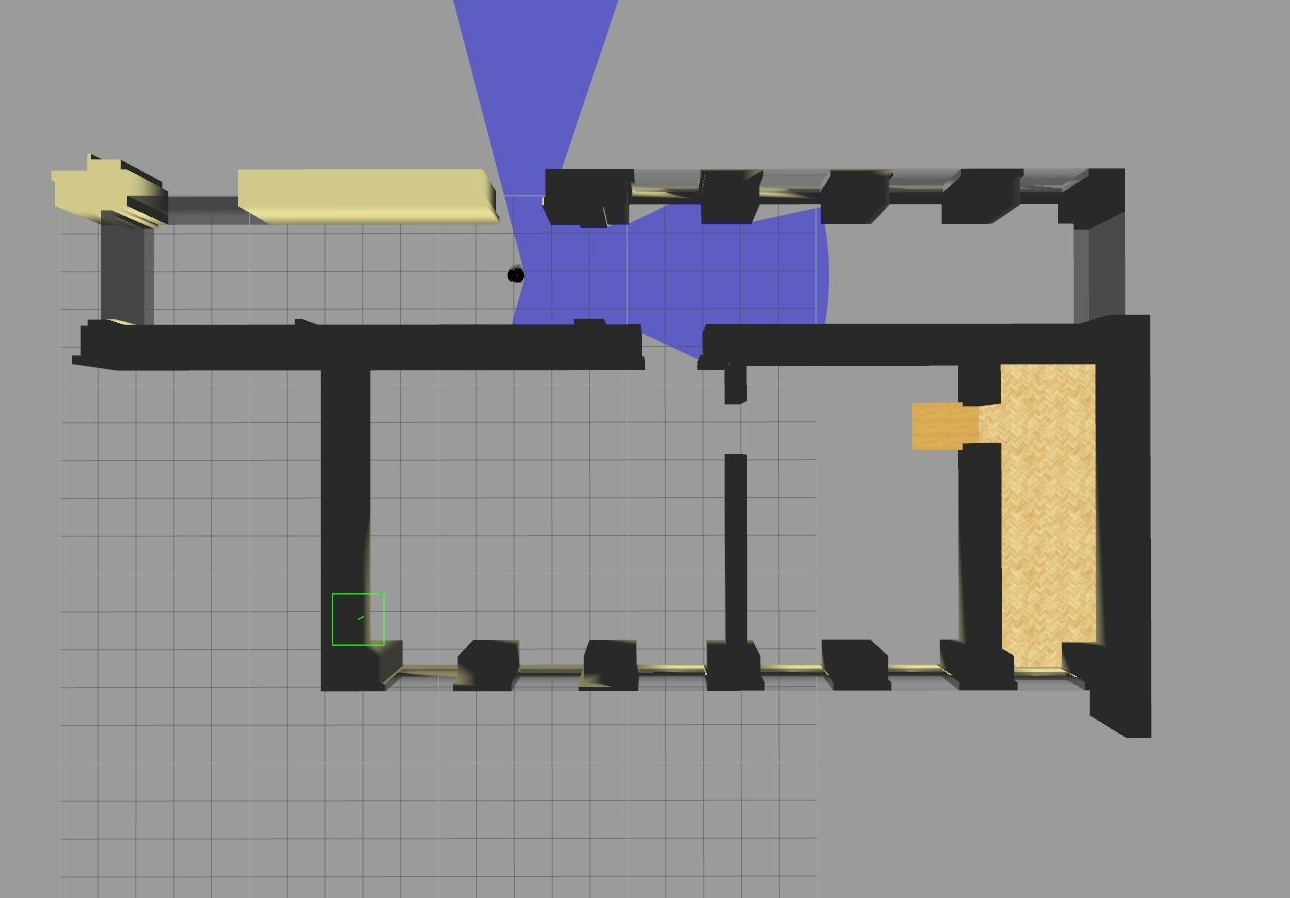
\includegraphics[width=\textwidth]{figures/fig_gh25_gazebo.jpg}}
       }\\
       \subfloat[]
       {  
           \fbox{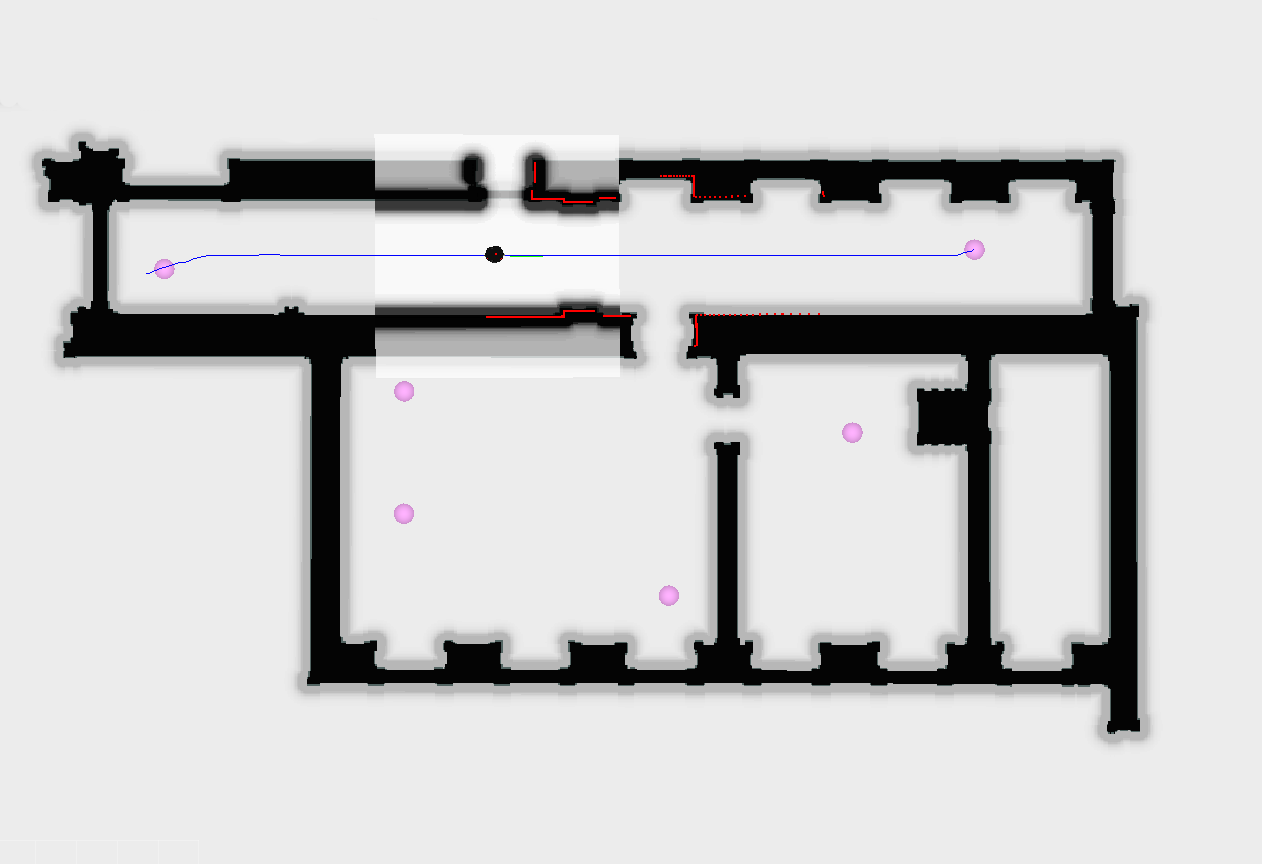
\includegraphics[width=\textwidth]{figures/fig_gh25_rviz.png}}
       }        
       \caption[Simulation: office environment]{Figure (a) shows the 3D model of an office environment used for the experiments with the simulation software Gazebo. Figure (b) depicts planning information used during the experiments.}
      \label{fig:gazebo_gh25}
   \end{figure}

To compare the meta-heuristic approach with the unaltered versions of the ROS-planners, a simulated robot has to fulfill a simple navigation task within the provided environments.
A route is provided by marker points which have to be approached one by one until a round trip is completed.
To account for the probability aspect of the meta-heuristic implementations several round trips have to be accomplished until the experiments stops.

At each call of the local planner first the original brute force evaluation of the trajectories is conducted and the best score together with the time needed to find the best trajectory is recorded.
Immediately after a solution is found, the VNS search algorithm searches for the same exact best score.
Again the performance time until completion of the algorithm is recorded.
The performance time of the original and the altered version of the local planner are used for  comparing the different algorithms. 

The following list shows the tested algorithm:
\begin{itemize}
\item{\bf{VNS-ROL:}} This implementation uses Variable Neighborhood Search with Best Improvement together with the Trajectory Roll-out planner.
\item{\bf{VNS-DWA:}} This implementation uses Variable Neighborhood Search with Best Improvement together with the Dynamic Window Approach planner. 
\end{itemize}

\section{Results}\label{sec:testresults}

All experiments account for the randomness of the proposed methods by running the algorithm multiple times.

The results are graphically visualized using box plots. 
The colored box is bounded by the lower quartile and the upper quartile of the data ($25\%$ and $75\%$ of the data). 
The median is indicated by a straight line through the box. 
The upper whisker extending at one end of the box indicate the last data point which lies below the $75\%$ quartile plus $1.5$ times the
inter quartile range (IQR). The lower whisker on the other end indicates the last data point which lies above the $25\%$ quartile minus 1.5 times the IQR. 
Points outside of the whisker range are considered outliers.
As a rule of thumb if the boxes between two measured data sets do not overlap, the difference between those data sets is significant.

Figure~\ref{fig:fig_boxplot} shows a commmon boxplot. 
%\begin{figure}[thpb]
\begin{figure}[thpb]
     \footnotesize
      \centering
       \def\svgwidth{\textwidth}
       \includesvg{figures/fig_boxplot}        
       \caption{A classical boxplot diagram.}
      \label{fig:fig_boxplot}
   \end{figure}

\subsection{Sample planner}
In this set of experiments the algorithms were tested using the sample planner and the artificial sensor map instances. 
These tests were performed on a 2.4 GHz, Intel Core 2 Duo processor using 4 GB RAM. 

\subsubsection{Influence of trajectory size}
The algorithms were applied to all 60 instances to evaluate a broad spectrum of possible environments. 
The main reason conducting this experiment is to get a first impression on the usefulness of applying meta-heuristics in the context of local planning. 
Figure~\ref{fig:fig_allworlds} illustrates the results using 240 trajectories, and using 2400 trajectory samples.

\begin{figure}[thpb]
   \myfloatalign
    \tiny
    \centering
   %\captionsetup[subfigure]{labelformat=empty} 
    \subfloat[]
    {  
       \def\svgwidth{0.75\textwidth}
       \includesvg{figures/fig_allworlds_6_40}
    }\\
    \subfloat[]
    {  
       \def\svgwidth{0.75\textwidth}
       \includesvg{figures/fig_allworlds_24_100}
    }
        \\
    {
    \captionsetup[subfigure]{labelformat=empty} 
    \subfloat[][] 
    {  
       \footnotesize
       \def\svgwidth{0.75\textwidth}
       \includesvg{figures/legend_all}
    }
    }
    \caption[Experiment: All instances]{This figure shows the results of testing all 60 randomly generated instances. The top figure shows the run time performance for 240 trajectories, and the bottom figure for 2400 trajectories. Compared to brute force search, the meta-heuristic algorithms show a significant improvement. (adapted from \cite{myself})}
      \label{fig:fig_allworlds}
   \end{figure}

The results show that all algorithms, including RST, outperform the Brute Force generate and test method significantly. 
As expected increasing the number of trajectories greatly favors the meta-heuristic algorithms, since they benefit from larger search spaces. 

Notice that ILS and VNS algorithms differ apparently from the RST by exhibiting much smaller variance in their test results, indicating that randomization alone is not enough to achieve very good and stable performance.
Furthermore the VNS exhibit a more stable performance than the ILS methods. 
Comparing the ILS algorithms reveals the connection of the search space size to the size of the neighborhood. 
A small number of trajectories benefits smaller sized neighborhoods, whereas increasing the number of trajectories benefits larger neighborhoods. 

\subsubsection{Influence of trajectory size by specific instances}
The following tests include the VNSF, VNSB and only one ILS4 algorithm for comparison. 
The algorithms are executed with specific world instances, and repeated 50 times. 
The results in Figure~\ref{fig:fig_special_240} show the application of the algorithm using 240 trajectories. Again  all tested algorithms significantly outperform the Brute Force method. 

\begin{figure}[thpb]
   \myfloatalign
    \tiny
          \centering
   %\captionsetup[subfigure]{labelformat=empty} 
    \subfloat[]
    {  
       \def\svgwidth{0.5\textwidth}
       \includesvg{figures/00_1_b_6_40}
    }
    \subfloat[]
    {  
       \def\svgwidth{0.5\textwidth}
       \includesvg{figures/15_3_b_6_40}
    }\\
    \subfloat[]
    {  
       \def\svgwidth{0.5\textwidth}
       \includesvg{figures/30_5_m_6_40}
    }
    \subfloat[]
    {  
       \def\svgwidth{0.5\textwidth}
       \includesvg{figures/32_5_m_6_40}
    }\\
    \subfloat[]
    {  
       \def\svgwidth{0.5\textwidth}
       \includesvg{figures/45_25_s_6_40}
    }
    \subfloat[]
    {  
       \def\svgwidth{0.5\textwidth}
       \includesvg{figures/51_25_s_6_40}
    }
    \\
    {
    \captionsetup[subfigure]{labelformat=empty} 
    \subfloat[][] 
    {  
       \footnotesize
       \def\svgwidth{0.5\textwidth}
       \includesvg{figures/legend_traj}
    }
    }
    \caption[Experiment: Specific instances with 240 trajectories]{The results of 50 consecutively executions with 240 trajectories. Plots (a,b) shows the result for 1 and 3 obstacles with size 1 meter. Plots (c,d) shows the result for 5 obstacles with size 0.5 meter, and plots (e,f) shows the result for 25 obstacles with size 0.1 meter. The blue line marks the run time for brute force search, which is used as a benchmark.(adapted from \cite{myself})}  
     \label{fig:fig_special_240}
\end{figure}

Increasing the number of trajectories favors the VNS algorithms over the ILS4 algorithm. The results in Figure~\ref{fig:fig_special_960} show the application of the algorithm using 960 trajectories.

\begin{figure}[thpb]
   \myfloatalign
    \tiny
          \centering
   %\captionsetup[subfigure]{labelformat=empty} 
    \subfloat[]
    {  
       \def\svgwidth{0.5\textwidth}
       \includesvg{figures/00_1_b_12_80}
    }
    \subfloat[]
    {  
       \def\svgwidth{0.5\textwidth}
       \includesvg{figures/15_3_b_12_80}
    }\\
    \subfloat[]
    {  
       \def\svgwidth{0.5\textwidth}
       \includesvg{figures/30_5_m_12_80}
    }
    \subfloat[]
    {  
       \def\svgwidth{0.5\textwidth}
       \includesvg{figures/32_5_m_12_80}
    }\\
    \subfloat[]
    {  
       \def\svgwidth{0.5\textwidth}
       \includesvg{figures/45_25_s_12_80}
    }
    \subfloat[]
    {  
       \def\svgwidth{0.5\textwidth}
       \includesvg{figures/51_25_s_12_80}
    }
        \\
    {
    \captionsetup[subfigure]{labelformat=empty} 
    \subfloat[][] 
    {  
       \footnotesize
       \def\svgwidth{0.5\textwidth}
       \includesvg{figures/legend_traj}
    }
    }
    \caption[Experiment: Specific instances with 960 trajectories]{The results of 50 consecutively executions with 960 trajectories. Plots (a,b) shows the result for 1 and 3 obstacles with size 1 meter. Plots (c,d) shows the result for 5 obstacles with size 0.5 meter, and plots (e,f) shows the result for 25 obstacles with size 0.1 meter. The blue line marks the run time for brute force search, which is used as a benchmark.(adapted from \cite{myself})}  
     \label{fig:fig_special_960}
\end{figure}
   
In contrast to the smaller number of trajectories, the results of the ILS4 algorithms shows that a too small environment will quickly degrade to random search if the number of trajectories increases. 
Here the use of a neighborhood structure pays off and the VNS approaches perform evidently better than ILS. 
In addition, the results show that the algorithms perform good independent of number and size of obstacles.

\subsubsection{Influence of velocity bounds}
The next analysis focuses on the influence of the velocity bounds on the performance of the local planning step. 
The trajectory size is fixed to 240 trajectories and the velocity bounds are varied.
Since the previous test has shown that the VNS approaches are more promising, the following experiments omit the ILS algorithms.
5 experiments with 50 runs and increasing acceleration windows are conducted.
The test are again performed on different sizes and numbers of obstacles.

In Figure~\ref{fig:fig_vel_big} the results on instances with 1 to 3 obstacle with size 1 meter are presented. 

Figure~\ref{fig:fig_vel_medium} presents the results on instances with 5 obstacles with size 0.5 meter.  

In Figure~\ref{fig:fig_vel_small} the results on instances with 25 obstacles with size 0.1 meter are presented.

\begin{figure}[thpb]
   \myfloatalign
    \tiny
          \centering
   %\captionsetup[subfigure]{labelformat=empty} 
    \subfloat[]
    {  
       \def\svgwidth{0.75\textwidth}
       \includesvg{figures/vel_comp_b_04_1}
    }\\
    \subfloat[]
    {  
       \def\svgwidth{0.75\textwidth}
       \includesvg{figures/vel_comp_b_19_3}
    }\\
    \subfloat[]
    {  
       \def\svgwidth{0.75\textwidth}
       \includesvg{figures/vel_comp_b_29_3}
    }
    \\
    {
    \captionsetup[subfigure]{labelformat=empty} 
    \subfloat[][] 
    {  
       \footnotesize
       \def\svgwidth{0.2\textwidth}
       \includesvg{figures/legend_vel}
    }
    }
    \caption[Experiment: Big obstacle instances with different velocity bounds]{The results of 50 consecutively executions with 240 trajectories, on instances with 1 (a) and 3 obstacles (b-c) with size 1 meter. The blue line marks the run time for brute force search, which is used as a benchmark.}  
     \label{fig:fig_vel_big}
\end{figure}

\begin{figure}[thpb]
   \myfloatalign
    \tiny
          \centering
   %\captionsetup[subfigure]{labelformat=empty} 
    \subfloat[]
    {  
       \def\svgwidth{0.75\textwidth}
       \includesvg{figures/vel_comp_m_30_5}
    }\\
    \subfloat[]
    {  
       \def\svgwidth{0.75\textwidth}
       \includesvg{figures/vel_comp_m_31_5}
    }\\
    \subfloat[]
    {  
       \def\svgwidth{0.75\textwidth}
       \includesvg{figures/vel_comp_m_44_5}
    }
    \\
    {
    \captionsetup[subfigure]{labelformat=empty} 
    \subfloat[][] 
    {  
       \footnotesize
       \def\svgwidth{0.2\textwidth}
       \includesvg{figures/legend_vel}
    }
    }
    \caption[Experiment: Medium obstacle instances with different velocity bounds]{The results of 50 consecutively executions with 240 trajectories, on instances with 5 obstacles with size 0.5 meter. The blue line marks the run time for brute force search, which is used as a benchmark.}  
     \label{fig:fig_vel_medium}
\end{figure} 

\begin{figure}[thpb]
   \myfloatalign
    \tiny
          \centering
   %\captionsetup[subfigure]{labelformat=empty} 
    \subfloat[]
    {  
       \def\svgwidth{0.75\textwidth}
       \includesvg{figures/vel_comp_s_47_25}
    }\\
    \subfloat[]
    {  
       \def\svgwidth{0.75\textwidth}
       \includesvg{figures/vel_comp_s_53_25}
    }\\
    \subfloat[]
    {  
       \def\svgwidth{0.75\textwidth}
       \includesvg{figures/vel_comp_s_58_25}
    }
    \\
    {
    \captionsetup[subfigure]{labelformat=empty} 
    \subfloat[][] 
    {  
       \footnotesize
       \def\svgwidth{0.2\textwidth}
       \includesvg{figures/legend_vel}
    }
    }
    \caption[Experiment: Small obstacle instances with different velocity bounds]{The results of 50 consecutively executions with 240 trajectories, on instances with 25 obstacles with size 0.1 meter. The blue line marks the run time for brute force search, which is used as a benchmark.}  
     \label{fig:fig_vel_small}
\end{figure}

All meta-heuristic algorithms outperform the Brute Force generate and test method on all tested instances, regardless of the differences in the velocity bounds.
It can be observed that the small instances with many obstacles provide the most difficulties for the proposed methods.
This is increased by using a larger velocity space.
While increasing the velocity windows clearly has an obvious negative effect on the performance of both the brute force and the meta-heuristic methods, the meta-heuristic algorithms soften this influence to a large degree. 

\subsection{Existing local planner}
This set of experiments are conducted using the simulation software Gazebo for the artificial and office environment. 
All of these tests are performed on an Intel Core2 Quad CPU with 2.66GHz and 8 GB RAM.

\subsubsection{VNS and Trajectory Roll-out planner}
The Trajectory Roll-out planner variant of the ROS-navigation stack implementation was altered to use the VNS approach (VNS-ROL) and compared to the unaltered version in all of the following results.

The first experiment was executed using only one tabu list which holds all visited solutions. 
The robot was tested with 300 trajectories in the logo environment and had to perform 15 roundtrips.
The results in figure~\ref{fig:fig_logo_rol_ori} show that the VNS-ROL algorithm significantly outperforms the original approach. 

In a second experiment the experiment time was extended to 80 roundtrips in the logo environment.
Again the local planner used 300 trajectories.
This time both memory structures were used with a tabu tenure of 7.
The results in figure~\ref{fig::fig_logo_rol2tabu} show again that the VNS-ROL algorithm significantly outperforms the original approach. 

\begin{figure}[thpb]
   \myfloatalign
    \tiny
    \centering
   %\captionsetup[subfigure]{labelformat=empty} 
    \subfloat[1-tabu] 
    {  
       \label{fig:fig_logo_rol_ori}
       \def\svgwidth{0.5\textwidth}
       \includesvg{figures/fig_logo_rol_ori}
    }
    \subfloat[2-tabu]    
    {  
       \label{fig::fig_logo_rol2tabu}
       \def\svgwidth{0.5\textwidth}
       \includesvg{figures/fig_logo_rol_2tabu}
    }
    \\
    {
    \captionsetup[subfigure]{labelformat=empty} 
    \subfloat[][] 
    {  
       \footnotesize
       \def\svgwidth{0.2\textwidth}
       \includesvg{figures/legend_rol}
    }
    }

    \caption[Experiment: VNS-ROL logo]{These figures show the result of using the VNS-ROL algorithm in the logo environment.
    The results of 15 roundtrips with one tabu list is shown in (a).  Figure (b) shows the result of 80 roundtrips using an additional tabu list with tenure 7.}  
     \label{fig:fig_logo_rol}
\end{figure} 

Using the short term memory structure did have a small but not significant performance increase, although less outliers and slightly smaller variance of the measurements is observable.  

The next four experiments show the effects of increasing the number of trajectory samples and the influence of the tabu tenure.
This time the robot had to travel 40 roundtrips in the office environment. The planners are tested with 300 and 600 trajectories with tabu tenure set to 10 and 100.
The results are shown in figure~\ref{fig:fig_gh25_rol}.
 
\begin{figure}[thpb]
   \myfloatalign
    \tiny
    \centering
    
    \subfloat[][trajectories=300, tenure=10] 
    {  
       \label{fig:fig_gh25_rol_2tabu_40_10_30_nb6_10}
       \def\svgwidth{0.5\textwidth}
       \includesvg{figures/fig_gh25_rol_2tabu_40_10_30_nb6_10}
    }
    \subfloat[][trajectories=300, tenure=100]    
    {  
       \label{fig::fig_gh25_rol_2tabu_40_10_30_nb6_100}
       \def\svgwidth{0.5\textwidth}
       \includesvg{figures/fig_gh25_rol_2tabu_40_10_30_nb6_100}
    }
    \\
    \subfloat[][trajectories=600, tenure=10] 
    {  
       \label{fig:fig_gh25_rol_2tabu_40_15_40_nb6_10}
       \def\svgwidth{0.5\textwidth}
       \includesvg{figures/fig_gh25_rol_2tabu_40_15_40_nb6_10}
    }
    \subfloat[][trajectories=600, tenure=100]    
    {  
       \label{fig::fig_gh25_rol_2tabu_40_15_40_nb6_100}
       \def\svgwidth{0.5\textwidth}
       \includesvg{figures/fig_gh25_rol_2tabu_40_15_40_nb6_100}
    }
    \\
    {
    \captionsetup[subfigure]{labelformat=empty} 
    \subfloat[][] 
    {  
       \footnotesize
       \def\svgwidth{0.2\textwidth}
       \includesvg{figures/legend_rol}
    }
    }


    \caption[Experiment: VNS-ROL office]{These figures show the result of using the VNS-ROL algorithm in the office environment. In each experiment the robot has to drive 40 roundtrips in the building. Figure (a) shows the result using 300 trajectory samples with tabu tenure 10 while Figure (b) uses a tenure of 100. Figure (c) shows the result of 600 trajectories with tabu tenure 10 and Figure (d) a tenure of 100.}  
     \label{fig:fig_gh25_rol}
\end{figure} 

As in the experiments with the sample planner, the larger trajectory size increased the performance difference between the original brute-force method and the VNS approach.
Increasing the size of the tabu tenure did have a negative effect on the performance, showing that a small tenure is not only enough to avoid cycling but is also faster due to the smaller lookup time in a shorter list.
 
\subsubsection{VNS and DWA planner}
This section contains the results of the experiments with the DWA variant of the ROS local planner and the VNS approach (VNS-DWA).

Starting with 15 roundtrips using 300 trajectories in the logo environment the meta-heuristic algorithm shows similar good performance as the  VNS-ROL algorithm. 

The long run experiment with 80 roundtrips revealed a problem for the VNS-DWA approach with 2 tabu lists, which was not detected during the tests with the Rollout planner.
In some rare cases the meta-heuristic approach did use exceptional long time to find the best solution, leading to instability of the system.
Even extending the tabu tenure to half of the solution size did not solve this problem.

Through further analysis the problem was identified to occur only when the robot approached a milestone in the roundtrip with very small velocity.
Since the robot did barely move at all the corresponding cost function had the same value for most velocity tuples, providing no usable gradient for guiding the local search. 

In order to avoid this situation the VNS-DWA algorithm was altered to use the brute force method whenever the velocity of the robot drops beyond a predefined very small threshold value.

The result of these experiments are shown in figure~\ref{fig:fig_logo_dwa}
\begin{figure}[thpb]
   \myfloatalign
    \tiny
    \centering
   %\captionsetup[subfigure]{labelformat=empty} 
    \subfloat[1-tabu] 
    {  
       \label{fig:fig_logo_dwa_ori}
       \def\svgwidth{0.5\textwidth}
       \includesvg{figures/fig_logo_dwa_ori}
    }
    \subfloat[2-tabu]    
    {  
       \label{fig::fig_logo_dwa2tabu}
       \def\svgwidth{0.5\textwidth}
       \includesvg{figures/fig_logo_dwa_2tabu}
    }
    \\
    {
    \captionsetup[subfigure]{labelformat=empty} 
    \subfloat[][] 
    {  
       \footnotesize
       \def\svgwidth{0.2\textwidth}
       \includesvg{figures/legend_dwa}
    }
    }

    \caption[Experiment: VNS-DWA logo]{These figures show the result of using the VNS-DWA algorithm in the logo environment.
    The results of 15 roundtrips with one tabu list is shown in (a).  Figure (b) shows the result of 80 roundtrips using an additional tabu list with tenure 7.}  
     \label{fig:fig_logo_dwa}
\end{figure} 


For the next experiments the robot had to travel 40 roundtrips in the office environment. 
The planners are tested with 300 and 600 trajectories with tabu tenure set to 10 and 100.
The results are shown in figure~\ref{fig:fig_gh25_dwa}.
 
\begin{figure}[thpb]
   \myfloatalign
    \tiny
    \centering
    
    \subfloat[][trajectories=300, tenure=10] 
    {  
       \label{fig:fig_gh25_dwa_2tabu_40_10_30_nb6_10}
       \def\svgwidth{0.5\textwidth}
       \includesvg{figures/fig_gh25_dwa_2tabu_40_10_30_nb6_10}
    }
    \subfloat[][trajectories=300, tenure=100]    
    {  
       \label{fig::fig_gh25_dwa_2tabu_40_10_30_nb6_100}
       \def\svgwidth{0.5\textwidth}
       \includesvg{figures/fig_gh25_dwa_2tabu_40_10_30_nb6_100}
    }
    \\
    \subfloat[][trajectories=600, tenure=10] 
    {  
       \label{fig:fig_gh25_dwa_2tabu_40_15_40_nb6_10}
       \def\svgwidth{0.5\textwidth}
       \includesvg{figures/fig_gh25_dwa_2tabu_40_15_40_nb6_10}
    }
    \subfloat[][trajectories=600, tenure=100]    
    {  
       \label{fig::fig_gh25_dwa_2tabu_40_15_40_nb6_100}
       \def\svgwidth{0.5\textwidth}
       \includesvg{figures/fig_gh25_dwa_2tabu_40_15_40_nb6_100}
    }
    \\
    {
    \captionsetup[subfigure]{labelformat=empty} 
    \subfloat[][] 
    {  
       \footnotesize
       \def\svgwidth{0.2\textwidth}
       \includesvg{figures/legend_dwa}
    }
    }


    \caption[Experiment: VNS-DWA office]{These figures show the result of using the VNS-DWA algorithm in the office environment. In each experiment the robot has to drive 40 roundtrips in the building. Figure (a) shows the result using 300 trajectory samples with tabu tenure 10 while Figure (b) uses a tenure of 100. Figure (c) shows the result of 600 trajectories with tabu tenure 10 and Figure (d) a tenure of 100.}  
     \label{fig:fig_gh25_dwa}
\end{figure} 

The VNS-DWA algorithm outperformed the original approach in all experiments.
Again the experiments with the larger trajectory samples favor the meta-heuristic approach.
In contrast to the results of the VNS-ROL experiments, the larger tabu tenure did not show to have any noticeable effect.

\section{Summary}
As it is the case for nearly all optimization problems, the No Free Lunch theorems \cite{wolpert1997no} apply also to the local planning domain. 
So it is no surprise that looking at all the results of the sample planner, there is no clear winner among the algorithms, but Variable Neighborhood search with tabu list and Best, or First Improvement heuristic seem to yields the best and most stable overall performance. 

In general the run time of the python implementation used for the example planner is not very efficient compared to tuned C++ implementations. 
Therefore the absolute numbers of the run time evaluations should be handled with care.

After analysis of the results with the sample python planner, the VNS approach is selected to be integrated into a navigation system based on a C++ implementation in the ROS framework.

The tests conducted with a simulation software show that the previous results carry over to a real navigation scenario. Extensions to the Trajectory Roll-out planner within the navigation stack of ROS using the VNS algorithm outperform the unaltered version significantly.

While the application of the VNS search for the Roll-out planner was straight forward, the tests revealed a problem with this approach for the DWA planner.
For very low velocities the corresponding costfunction did not provide enough information for a fast local search, leading to instability of the system.
In order to deal with these situations, the VNS-DWA algorithm falls back to brute force evaluation of trajectories whenever the robots moves very slow. 

After this small change the VNS-DWA could be successfully tested and the results showed, that the performance increase was still significant.

\section{Implementation Details}
The example planner was implemented using \emph{python} version $2.7$ (available at \url{http://python.com}). This allows for a fast prototype implementation of a local planner without the overhead and interruption of other parts of full planning systems.
Hence the optimization algorithms could be evaluated focusing on the  specific trajectory selection part. 

For visualization, geometry related processing, and the creation of test scripts the python packages \emph{Numpy} (available at \url{http://numpy.org}), \emph{Python Imaging Library} (available at \url{http://pythonware.com}) and \emph{Matplotlib} (available at \url{http://matplotlib.org}) were an essential part of the created software. 

The VNS algorithm used in the navigation framework within ROS, was created using C++ and the BOOST-C++ Libraries (\url{http://boost.org}).

The source code was compiled using \emph{GCC} $4.6.4$ with optimization enabled.

Without the use of these exceptional open-source libraries the work presented in this thesis would not have been possible.  

 

